For these purposes, data is a point cloud (a finite set of points in some Euclidean space). Sometimes, though, as in DNA sequences, data isn't strictly a point, but rather a sequence. In ither case, a distance metric exists: the usual distance metric in Euclidean space, and the Hamming distance for sequences, which measures by how many points a sequence differs. Distance can be used to represent data, which leads to a notion of shape.

Shape of course is very relevant to data. For example, the most primitive notion of shape is whether the data clusters, which admits important statistical consequences. In general, shape represents some connected components; $\pi_0(x)$ denotes the set of connected components.
\begin{figure}[h!]
\centering
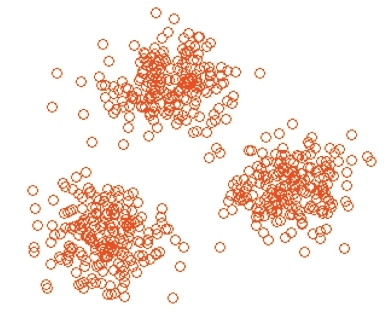
\includegraphics[width=2in]{clustering}
\caption{An example of data clustering into 3 different clusters.}
\end{figure}
Shape can also take the form of loops or other devices that represent periodic or recurrent behavior (as in the Lodka-Volterra predator-prey model), denoted $\pi_1(x)$ or $H_1(X)$, or flares, which indicate different ways in which the data can be an outlier, denoted $\pi_0^\infty(x)$.

In topology, one constructs invariants that measure this sort of shape. For $\pi_0(x)$, choose some distance $R$ and build a network (or simplicial complex; fill in all possible triangles, tetrahedra, etc.) connecting any two points with distance less than $R$. This actually builds up connected components from discrete sets, but distance must be chosen with care, or one obtains too many or too few clusters; choosing the proper $R$ can be an art. In statistics, heuristics exist, but there are plenty of counterexamples that limit their validity. However, a dendrogram (see Section~\ref{dendrogram}) can be helpful here.

Let $V(X,R)$ be the simplicial complex such that $x_i,x_j\in X$ are connected iff $d(x_i,x_j) \le R$. Thus, for every $R$, there is a set $\pi_0(V(X,R))$ of connected components at that fineness. If $R'<R$, then there exists a map $\pi_0(V(X,R))\to \pi_0(V(X,R'))$ because the latter is a subcomplex of the former (in a sense, it's more difficult to be a complex in $R'$). Thus, one can draw maps and points, leading to the familiar notion of a dendrogram. if the number of components remains constant over a long distance, then that suggests a correlation worth investigating.

Anothr method of doing this involves a homological method of shape. For every $k\ge 0$ and space $X$, one can associate a vector space on $\mathbb F_2$\footnote{$\mathbb F_2$ is sometimes called the Boolean space because its addition operation is equivalent to logical \texttt{xor} and its multiplication to logical \texttt{and}.} $H_k(X)$ such that $\dim H_k(X) = \beta_k$, where $\beta_k$ is the $k^{\mathrm{th}}$ Betti number.

$\beta_0$ is the number of connected components in $X$, and $\beta_1$ is the number of independent loops in $X$, so, for example $\beta_1(S^1) = 1$, and the first Betti number of two circles joined at a point is 2. Similarly, $\beta_1(T^2) = 2$, since there are two independent loops, but $\beta_1(S^2) = 0$, since all loops on $S^2$ can be shrunk to a point. Though these seem imprecise, rigorous foundations exist, and Betti numbers can be computed with methods from linear algebra.

%Have you added pictures yet?
$H_k$ is functional in that if $f:X\to Y$ is continuous them $H_k(X)\to H_k(Y)$ is an induced linear map. Apply it to $V(X,R)$, since the Betti numbers can change as $R$ imcreases (both increasing and decreasing; when nine points are separate, $\beta_1 = 0$, but when they become homeomorphic to a circle, $\beta_1 = 1$. When they are all connected again, $\beta_1 = 0$ again). In particular, for incomplete data, the Betti numbers might notice gaps or otherwise return the wrong result. Thus, one can do something similar and let $W_R = H_1(V(X,R))$ (some vector space over $\mathbb F_2$ and $W_R\to W_{R'}$ when $R < R'$ (due to the functoriality of the homology construction), which makes it necessary to find invariants on these persistence vector spaces.

These persistence spaces can be classified by ``bar codes'' (finite numbers of intervals). The category of persistence vector spaces happens to be equivalent to a certain category of rings for which an analogue to the Fundamental Theorem of Modules over Principal Ideal Domains (a generalization of Theorem~\ref{fgagtheorem}) holds, so some algebra comes over to help. If the barcodes contain  particularly long intervals, one can use them to classify things that are likely to be more meaningful. This is analogous to the dendrogram but involves loops rather than clustering.

One can apply this to statistics, but care must be taken --- it isn't practical for sufficiently complicated data sets, and point clustering may be ineffective. However, one can study similar problems or subproblems. For example, it is incredibly difficult to study all images of a given size, but one can study $3\times 3$ patches of images. Further refinement can be made because most pictures are dominated by constant patches, which can easily be removed. Thus, one looks at high-contrast patches of images that are normalized with respect to the mean (for intensity) and the $L^2$ norm (which represents contrast). This set $\mathcal M$ is dense in $S^7$, which is a little easier to work with. However, the density varies. This can be estimated (generally by counting the number of data points in a ball of a certain radius). If one considers the 25\% if the sphere with the largest density, there are always 5 intervals in the bar code, which was unexpected. However, this does correspond to a three-circle structure, with a primary circle that intersects two secondary circles (which do not intersect each other).

In order to simplify the problem further, one can represent this on a 2-dimensional surface: the Klein bottle. One can construct probability distributions and therefore Fourier analysis on the Klein bottle, which makes processing information nice. Thus this abstract Klein bottle can be used for very concrete applications.
